% !TEX program = lualatex
% !TEX options = -synctex=1 -interaction=nonstopmode -file-line-error -shell-escape -output-directory=%OUTDIR% "%DOC%"

\documentclass[12pt, a4paper]{article}
\usepackage{amsfonts}
\usepackage{amssymb}
\usepackage{amsmath}
\usepackage[english]{babel}
\usepackage{caption}
\usepackage{float}
\usepackage[left=2cm, top=2cm, right=2cm, bottom=2cm]{geometry}
\usepackage{graphicx}
\usepackage{listings}
\usepackage[newfloat, outputdir=out_tex]{minted}
\usepackage{pgf}
\usepackage{pdfpages}

\begin{document}
  \centerline{\Huge\scshape Computational physics}
  \vspace*{0.5cm}
  \hrule
  \vspace*{0.5cm}
  \centerline{Jona Ackerschott, Julian Mayr}
  \vspace*{1cm}
  \centerline{\Large\bfseries Problem set 4}
  \vspace*{0.5cm}

  \section*{Problem 1}
  Copying the given Mathematica code into our own notebook returns a plot of the numerical solution
  
  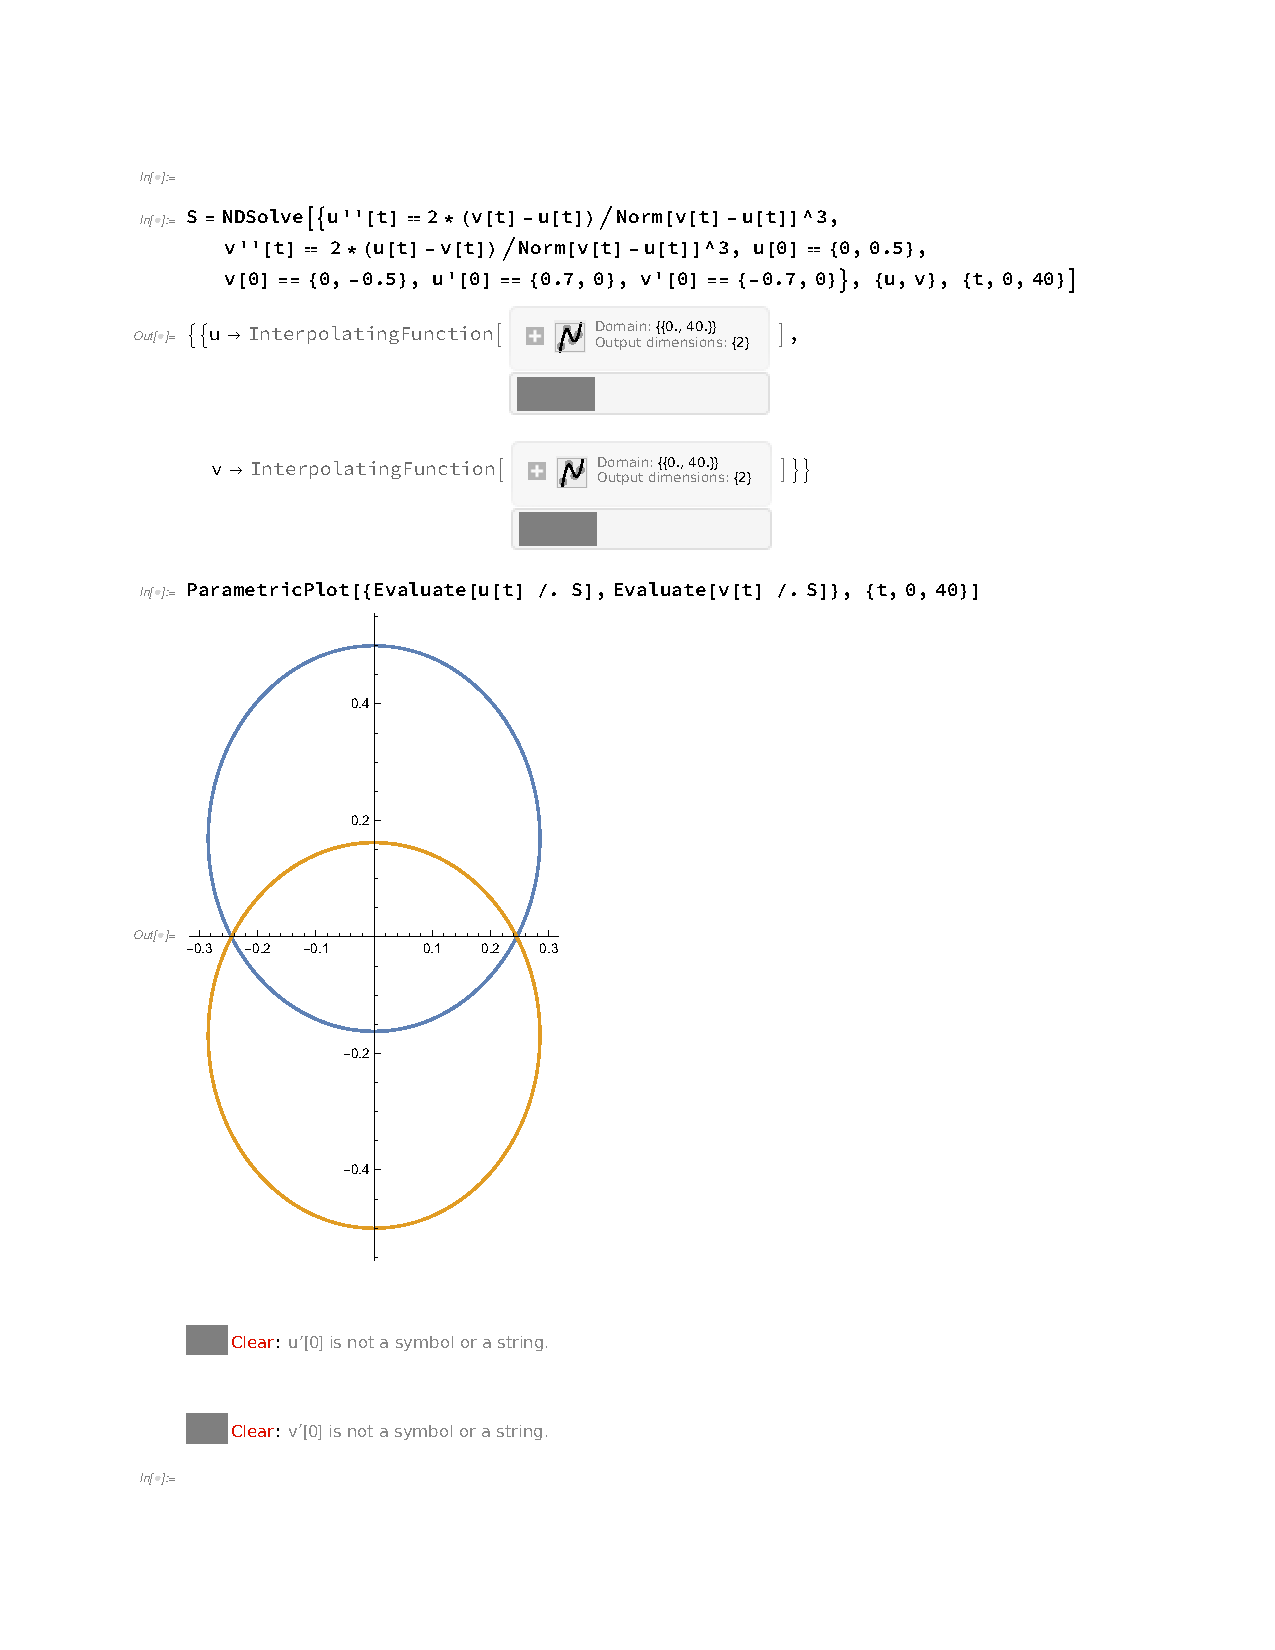
\includepdf[scale=0.7,pages=-,pagecommand=\subsection{]{2body.pdf}
  
  \section*{Problem 2}
  Through examination of the population dynamics equation
  \begin{align}
    \frac{{\rm d} N}{{\rm d} t} = r N (1 - N / K) - \frac{B N^2}{A^2+N^2}
    \label{eq_pop}
  \end{align}
  one sees immediately, using the dimensions of N (no dimension) and t
  (seconds) that $[r] = 1/{\rm s}$, $[K] = 1$, $[A] = 1$ and $[B] = 1/s$.
  So with the definitions $\varrho = r / B$ and $\tau = B t$ one obtains a
  dimensionless form of (\ref{eq_pop}).
  \begin{align}
    \frac{{\rm d} N}{{\rm d} \tau} = \varrho N (1 - N / K)
      - \frac{N^2}{A^2 + N^2}
  \end{align}
  Although this form already is dimensionless, here, $n = N / A$ is used
  as the \glqq dimensionless form\grqq{} of $N$, such that
  \begin{align}
    \frac{{\rm d} n}{{\rm d} t} = \varrho n \left(1 - \frac{A}{K} n\right)
      - \frac{1}{A} \frac{n^2}{1 + n^2}
  \end{align}

  \begin{align}
    & \varrho n \left(1 - \frac{A}{K} n \right)
      - \frac{1}{A} \frac{n^2}{1 + n^2} = 0 \nonumber \\
    \Leftrightarrow \ & \varrho n \left(1 - \frac{A}{K} n + n^2
    - \frac{A}{K} n^3 \right) - \frac{n^2}{A} = 0 \nonumber \\
    \Leftrightarrow \ & 
  \end{align}

\end{document}
